%%%%%%%%%%%%%%%%%%%%%%%%%%%%%%%%%%%%%%%%%
% Lachaise Assignment
% LaTeX Template
% Version 1.0 (26/6/2018)
%
% This template originates from:
% http://www.LaTeXTemplates.com
%
% Authors:
% Marion Lachaise & François Févotte
% Vel (vel@LaTeXTemplates.com)
%
% License:
% CC BY-NC-SA 3.0 (http://creativecommons.org/licenses/by-nc-sa/3.0/)
% 
%%%%%%%%%%%%%%%%%%%%%%%%%%%%%%%%%%%%%%%%%

%----------------------------------------------------------------------------------------
%	PACKAGES AND OTHER DOCUMENT CONFIGURATIONS
%----------------------------------------------------------------------------------------

\documentclass{article}

\input{structure.tex} % Include the file specifying the document structure and custom commands

\usepackage{etoolbox}
\patchcmd{\thebibliography}{\section*{\refname}}{}{}{}

%----------------------------------------------------------------------------------------
%	ASSIGNMENT INFORMATION
%----------------------------------------------------------------------------------------

\title{Project Proposal: Comparison of Real-Time Shadow Map Techniques (Percentage-Closer Filtered Hard Shadows and Percentage-Closer Soft Shadows)} % Title of the assignment

\author{Vincent Marias\\ \texttt{vmarias@mines.edu}} % Author name and email address 

\date{CSCI 544 --- Advanced Computer Graphics\\Colorado School of Mines\\\today} % University, school and/or department name(s) and a date

%----------------------------------------------------------------------------------------

\begin{document}

\maketitle % Print the title

%----------------------------------------------------------------------------------------
%	INTRODUCTION
%----------------------------------------------------------------------------------------

\section{Description} % Unnumbered section

Shadows are one of the most important components of a realistic computer-generated image. They provide crucial information about the spatial relationships of objects and lights in a scene. Without them, our brains can have a difficult time interpreting the final image. Unfortunately, they are also one of the most difficult components to render using rasterization. There are dozens of different shadowing techniques, varying widely in their accuracy, quality, and compute/memory consumptions. In general, the main categories break down into \textbf{hard shadows} and \textbf{soft shadows}, the difference being that soft shadows have variable-size penumbrae.

For my project, I will learn and implement from scratch two of the simplest (and importantly, \emph{cheapest}) methods, one for hard shadows and one for soft shadows, and compare the results.

\subsection{Percentage-Closer Filtering}

Starting with \textbf{hard shadows}, we can implement basic shadow mapping. This is a multi-pass technique where we first render the scene from the perspective of the light source, storing the depth buffer data to a texture. In the second pass, we compare the depth of each fragment rendered from the camera's perspective to the values in the texture. Put simply, if a fragment is further from the light source than the corresponding fragment in the camera's depth buffer, we say that it is occluded by the latter fragment, and is in shadow.

This produces very sharp, well-defined shadows, which are uniformly dark throughout. This is, of course, not accurate to real-life shadows which have both an umbra and penumbra. But it can be a "good-enough" solution if resources are limited. Now, as with any texturing technique, the problem becomes aliasing and sampling. And as with general texturing, we can perform some filtering. Percentage-closer filtering is a simple technique where we use some kernel to sample multiple times from the surrounding texels in the shadow map for each fragment and blend the results.

\subsection{Percentage-Closer Soft Shadows}

PCSS is one of the fastest techniques for soft shadows, as it works as a direct extension of the above PCF. If you vary the size of the PCF kernel, you'll notice that as it gets larger, the shadows get softer. This makes sense, as we're sampling and blending more of the surrounding depth values, and more of the fragments near the shadows edge will be part of this blurring process. So what if we adaptively updated the size of the PCF kernel for different parts of the shadow? In this way we could approximate the varying size of a shadow's penumbra.

So that's exactly what we'll do! Given the light size and the distances of the blocker and receiver from the light, if we assume each exists in parallel planes, we can use simple geometry to approximate the size of the penumbra. Based on this we can set the size of the PCF kernel, perform one step of filtering, and repeat for the remaining fragments. This gets us pretty good soft shadows with a single shadow map (per light source).

%----------------------------------------------------------------------------------------
%	PROBLEM 1
%----------------------------------------------------------------------------------------

\section{Application} % Numbered section

Shadows can (and should) be used in almost any 3D graphics application, even those not targeting a realistic visual style. They go a long way toward "grounding" a scene, providing depth and positioning information that is difficult for humans to infer otherwise. An application where you might \emph{not} want to use shadows could be in CAD or modeling software, where being able to see every part of the model clearly might be more important than realism.

For a long time, PCF hard shadows reigned supreme as the best solution for real-time applications like games. It was fast and simple, and more often than not it was "good-enough," especially when playing games at low resolutions. The issues with this approach are well-documented and understood, and solutions and optimizations abound.

PCSS is a slightly more modern technique, making it's way to triple-A games around 2015. It's more expensive than filtered hard shadows, but the uplift in accuracy and visual quality is immense. It's also one of the cheapest ways to get soft shadows, which are much more physically accurate than hard shadows, so it's can be a good choice for simulations and other real-time applications where realism might be important. There are also well-developed implementations provided to programmers by graphics APIs like NVIDIA GameWorks, that can be easy drop-in solutions for game engine development.

%----------------------------------------------------------------------------------------
%	PROBLEM 2
%----------------------------------------------------------------------------------------

\section{Challenge}

Using shadow maps, many problems arise when sampling them. These include shadow acne, peter panning, over-sampling, and aliasing. We are effectively reconstructing a signal from a lower-resolution representation, and so artifacts like these are common. There are plenty of methods for mitigating the effects of these artifacts, such as variance shadow maps, cascaded shadow maps, and even shadow volumes which represent an entirely different way of rendering shadows.

When implementing PCF itself, the main challenge is choosing and appropriately applying a kernel. A standard nearest-neighbor kernel will produce better shadows, but the aliasing is still present and still has a regular pattern. There are other kernels to try such as bilinear, Poisson disk, interleaved, and adaptive sampling. These all produce different results, and getting the best shadows becomes an exercise in choosing the right kernel for your application, and dealing with noise in a visually satisfying way. For example, we could introduce irregular noise into the Poisson disk sampling method by randomly rotating the disks.

Being an extension of PCF, PCSS has all the same problems. The added challenge is now in how you implement the steps of this method's algorithm. The way in which the blocker search step is performed, for example, changes the results of the following steps. The final PCF filter size must be proportional to the estimated penumbra size, but that doesn't give us any hard and fast rules on the magnitudes to be used.

%----------------------------------------------------------------------------------------
%	INTRODUCTION
%----------------------------------------------------------------------------------------

\section{Existing Work Survey} % Unnumbered section

Luckily for me, much has been written about both of these techniques, and shadows in general. For my basic understanding of how they work (as I've described them above), I read several sections of the book "Real-Time Shadows" by Eisemann et al \cite{eisemann2011real}. and the article on "Shadow Mapping" from LearnOpenGL.com, written by Joey de Vries \cite{de2015learn}. These provide plenty of information about PCF for me to implement it myself. You can see what the most basic implementation of this method will look like in Figure 1. Those images are from LearnOpenGL.com, where the most simple nearest-neighbor kernel is used. I will likely start with this kernel and branch out from there, to compare the different results. The website does provide their source code, but I won't be using it for anything other than reference (I don't like the way the author writes their code). The chapters in "Real-Time Shadows" describe more of the theory and math behind the technique, including several different types of kernels and ways to optimize the algorithm.

\begin{figure}
	\includegraphics[width=.49\linewidth]{images/hard_shadows_no_filtering}\hfill
	\includegraphics[width=.49\linewidth]{images/hard_shadows_no_filtering_closeup}
	\\[\smallskipamount]
	\includegraphics[width=.49\linewidth]{images/hard_shadows_pcf}\hfill
	\includegraphics[width=.49\linewidth]{images/hard_shadows_pcf_closeup}
	\caption{Hard shadows without filtering [top] vs. with percentage-closer filtering applied [bottom]. (\url{https://t.ly/qlob-/})}
\end{figure}

PCSS will be a bit more difficult, as there aren't a lot of easy-to-follow tutorials like the ones on LearnOpenGL.com that describe the exact implementation. There is some information in "Real-Time Shadows," as well as antoher book I have called "Real-Time Rendering" by Tomas Akenine-Möller et al. \cite{akenine2019real}. Again, these sources describe the theory of the method, and provide a lot of insight into how one might go about implementing it, but they don't explicitly show me any of the code used in implementation. I also read the original paper introducing PCSS by Randima Fernando \cite{ctx12351924680002341}, which is incredibly short. It does have some excellent figures that helped me understand how the method works, though.

My goal is to implement PCSS on my own just by understanding the theory, but if that proves to be too difficult or I get stuck somewhere, I found an online tutorial by a programmer named Andrew Pham \cite{pham_2020} that goes through at least some of the shader code which I could reference.

It's not exactly a research source, but I'd be remiss not to mention that the reason I chose PCSS for my project is because it was used (actually added after the fact in a patch) in one of my favorite games, Dying Light, back in 2015. I thought the result in-game looked really good and I wanted to try doing the same thing myself. In Figure 2, you can see screenshots from the game showing off NVIDIA's implementation of PCSS in action. Notice how the shadows harden as they get closer to and come into contact with the object casting them, and get softer as they get further from the object. It's especially noticeable on the shadows of the palm trees, which were weirdly sharp even at extreme distances from the trees casting them in the original version of the game.

\begin{figure}
	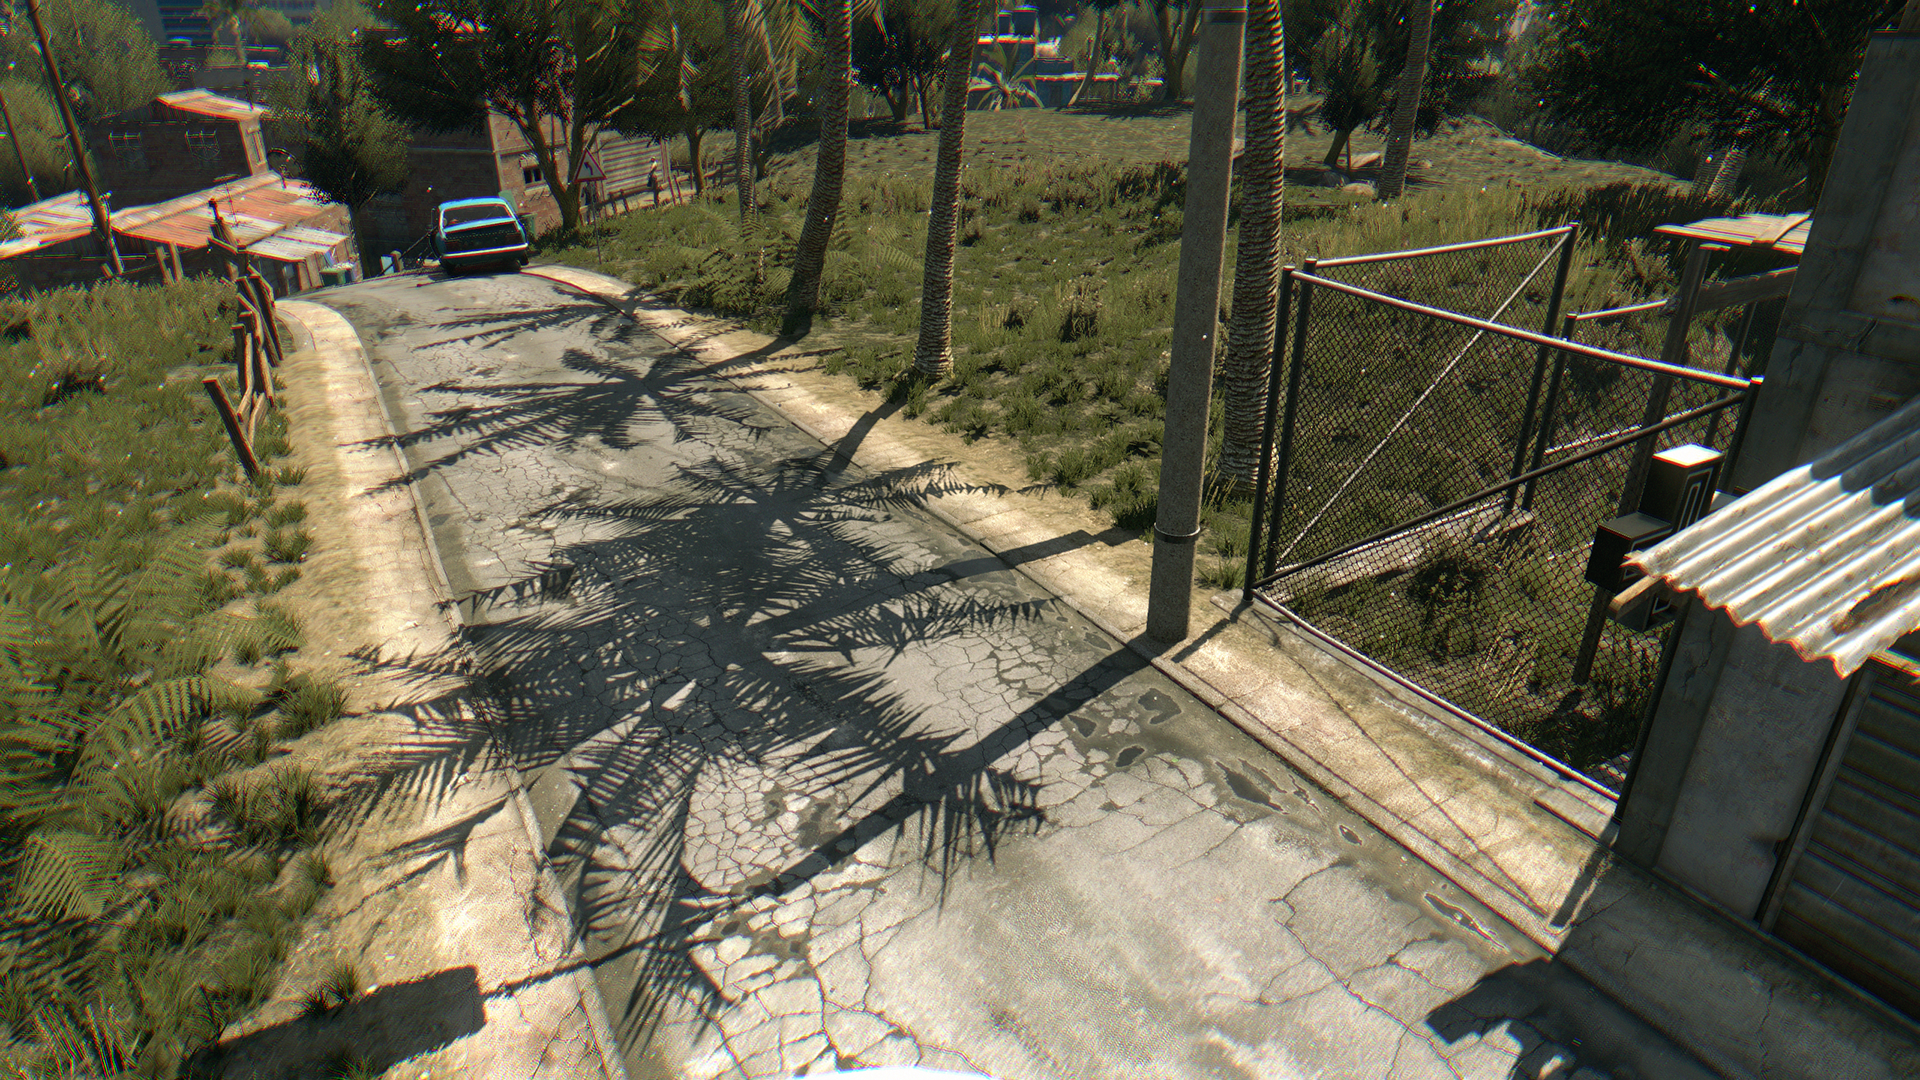
\includegraphics[width=.49\linewidth]{images/dying-light-pcss-001-off}\hfill
	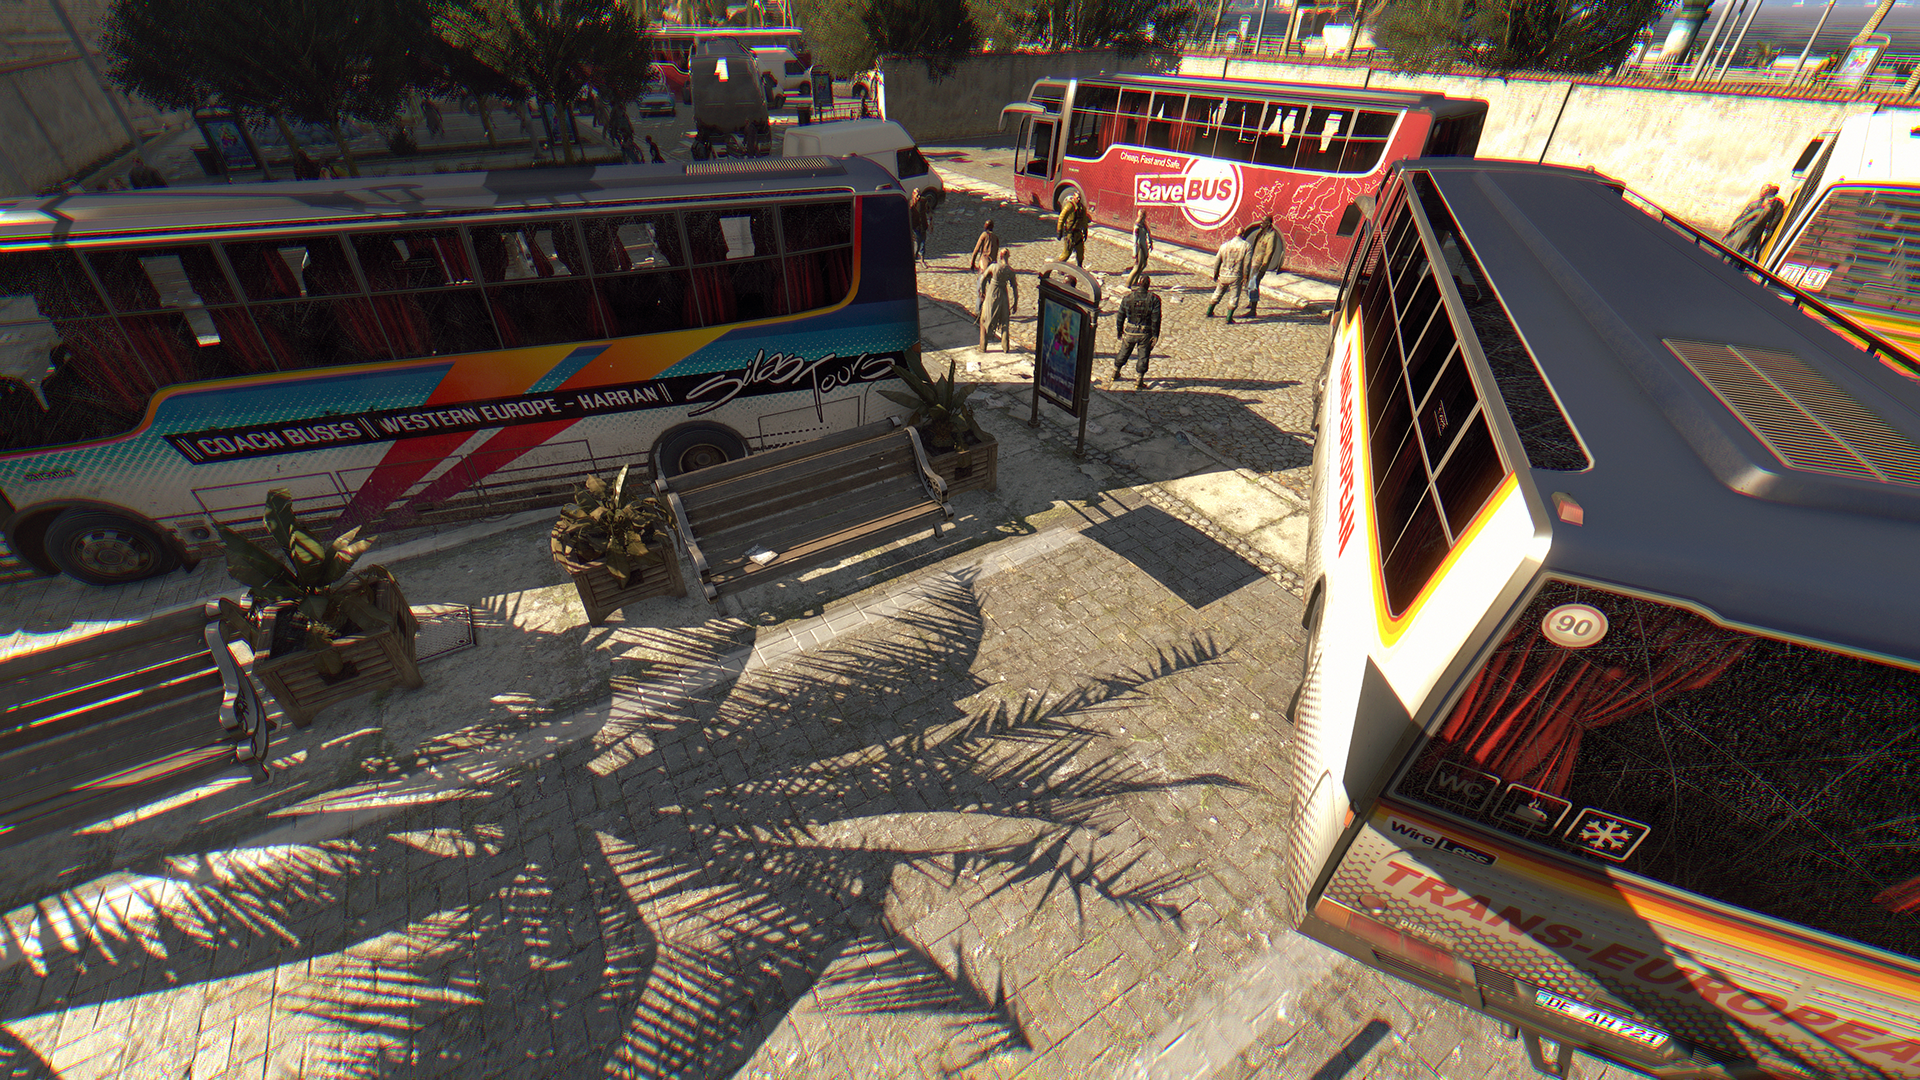
\includegraphics[width=.49\linewidth]{images/dying-light-pcss-003-off}
	\\[\smallskipamount]
	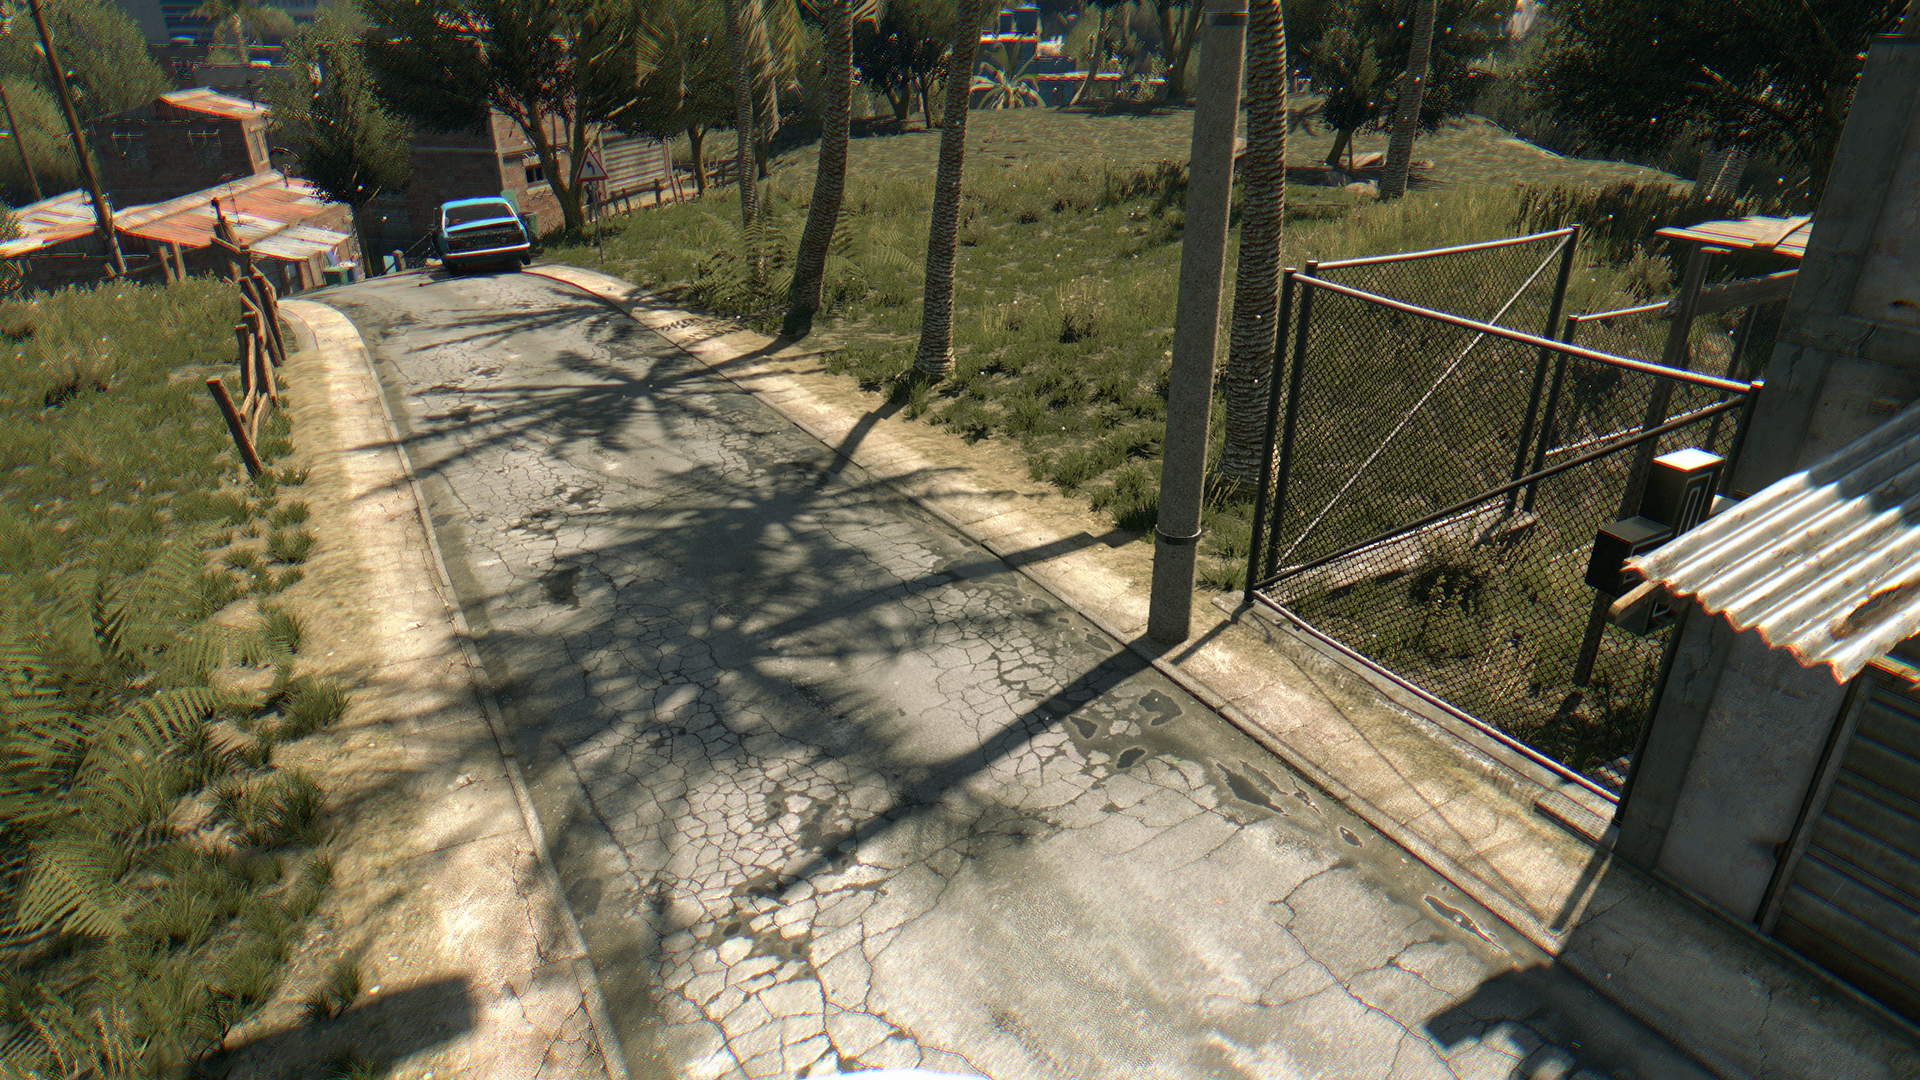
\includegraphics[width=.49\linewidth]{images/dying-light-pcss-001-on}\hfill
	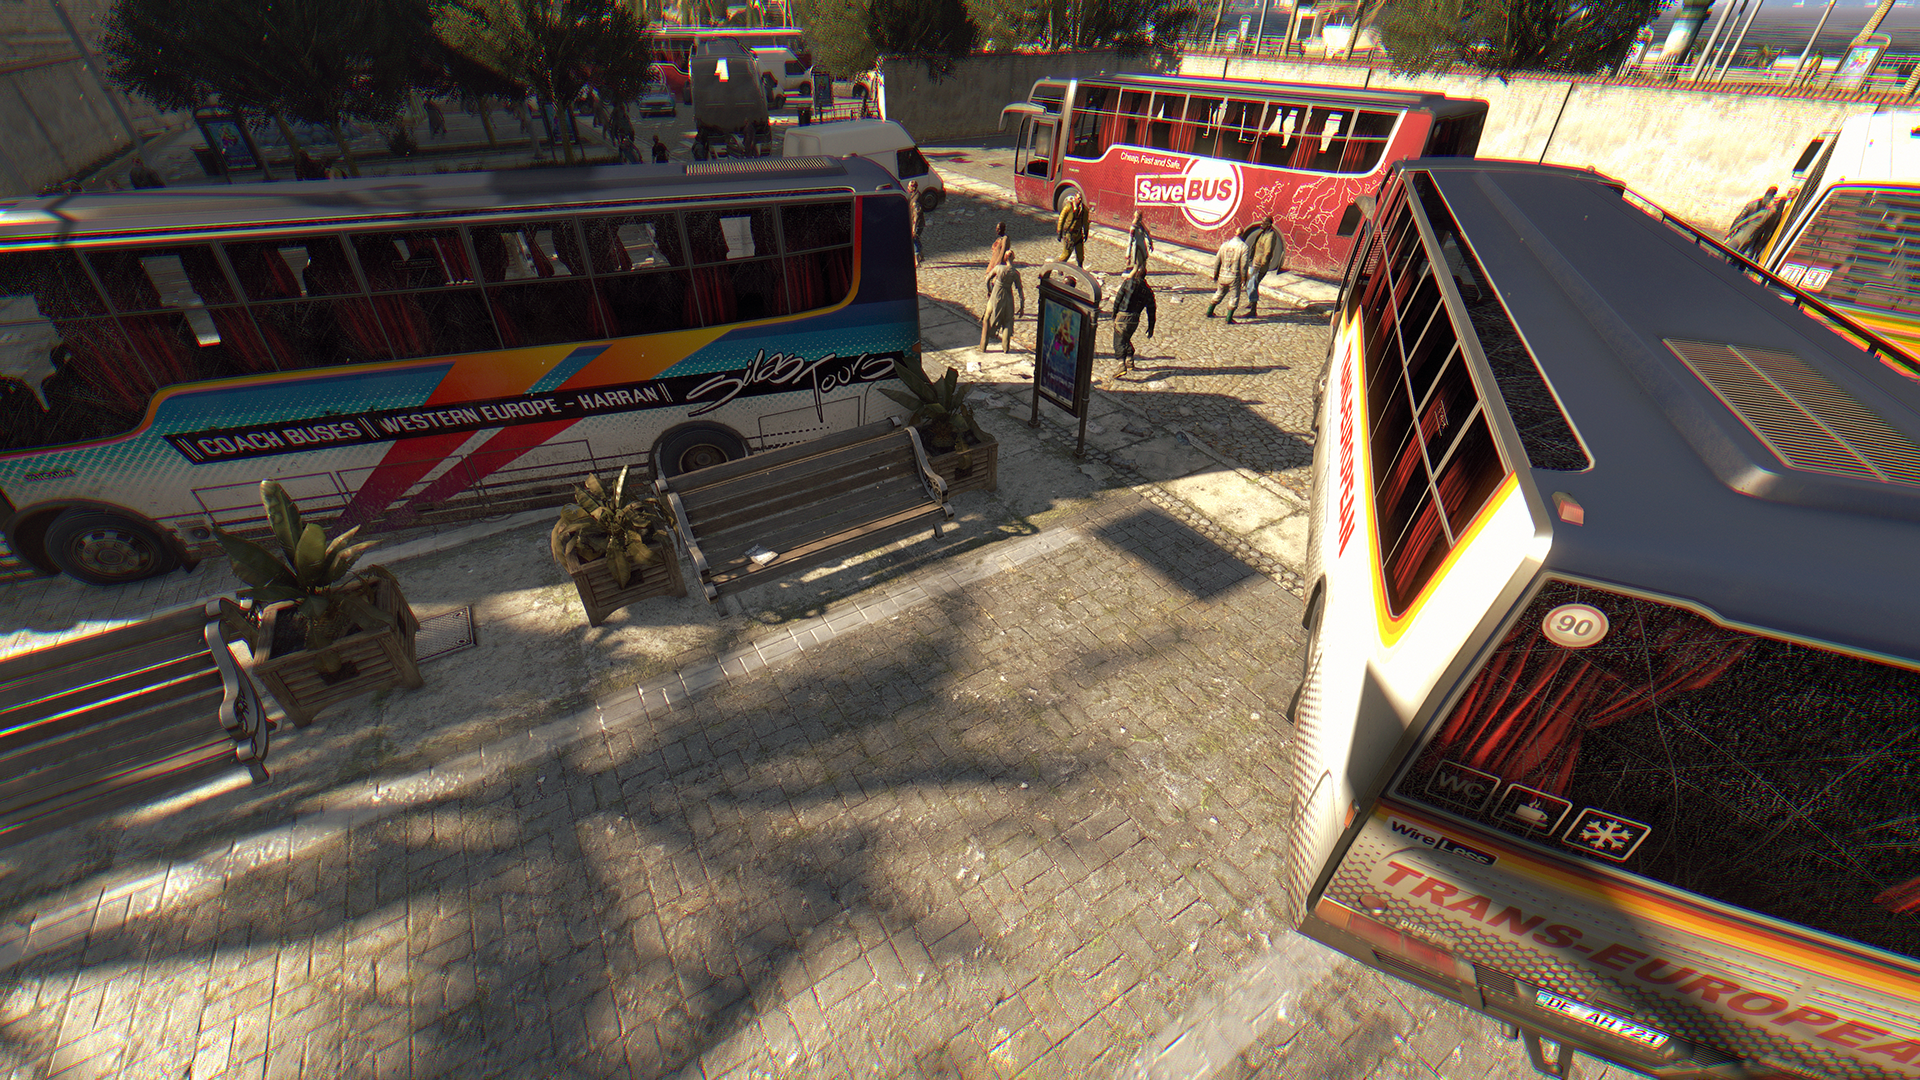
\includegraphics[width=.49\linewidth]{images/dying-light-pcss-003-on}
	\caption{Traditional hard shadows [top] vs. NVIDIA GameWorks Percentage-Closer Soft Shadows [bottom] as seen in Dying Light (2015). (\url{https://t.ly/kzboU/})}
\end{figure}

%----------------------------------------------------------------------------------------
%	INTRODUCTION
%----------------------------------------------------------------------------------------

\section{References / Sources} % Unnumbered section

\bibliography{sources}
\bibliographystyle{ieeetr}

%----------------------------------------------------------------------------------------

\end{document}
